\documentclass[conference]{IEEEtran}
\usepackage{amsfonts}
\usepackage{graphicx}
\usepackage{tabularx}
\usepackage{amsmath}
\usepackage{caption}
\ifCLASSINFOpdf
\else
\fi
\hyphenation{op-tical net-works semi-conduc-tor}
\begin{document}
\title{Handwritten Character Recognition}
\author{\IEEEauthorblockN{Gaurav Krishna}
\IEEEauthorblockA{gkrishna@iitk.ac.in}
\and
\IEEEauthorblockN{Harshit Maheshwari}
\IEEEauthorblockA{harshitm@iitk.ac.in}
\and
\IEEEauthorblockN{Pulkit Jain}
\IEEEauthorblockA{pulkitj@iitk.ac.in}\and
\IEEEauthorblockN{Sayantan Marik}
\IEEEauthorblockA{smarik@iitk.ac.in}}
\maketitle


\begin{abstract}
	Handwritten character recognition refers to task of classifying a given handwritten character (generally given as an image), into one of the elements of the alphabet.  The alphabet here consists of the 62 alphanumeric characters in English \{0-9, a-z, A-Z\}. In this report, we aim to produce comparative results obatined by trying out several of the existing methods for classification.
\end{abstract}

\section{Introduction}
Handwritten character recognition is a challenging classification task that has been studied extensively and remains an active area of research. The toughness in the task arises due to the large variability that arises amongst handwritten characters in the form of shape and size of character, the thickness of strokes, edges and curvatures. The task can be primarily classified into two classes

\subsection{Online Character Recognition}
This involves automatic conversion of text as it is written on touch interface of some tablet or some PDA(personal digital Assistant). The recognizer converts the sensor input from touch interface into characters which are usable in text processing application and typically styles and touch sensitive surfaces are combined with such kind of online character recognizer. 

\subsection{Offline Characted Recognition}
This involves conversion of images/scanned copies of handwritten documents into soft copies which can be processed by text processing applications. 
The main difference between the two is that offline recognizer uses static data while in online charcter recognition we get data dynamically. 
The problem statement that we are addressing in our project involves offline character recognition techniques.

\section{Literature Review}

Some of the methods that have been tried for the task of handwritten digits include K-nearest neighbours, SVMs, neural nets, and convolution neural networks. [1] presents a table showing comparative results over the classification task over the MNIST digits dataset. The dataset consists of about 60000 training examples and 10000 test examples. We present some of the results from [1] in the Table 1.
\newline\newline
\bgroup
\def\arraystretch{1.5}
\begin{table}[h]
\centering
\caption{Classification results over MNIST digits from [1]}
\begin{tabularx}{0.5\textwidth}{lcc}\hline\hline
Method & Preprocessing & Error Rate \\
\hline
K-NN (Eucledian) & None & 5\\
40PCA + quadratic & None & 3.3\\
1000 RBF + linear & None & 3.6 \\
SVM deg 4 polynomial & Deskewing & 1.1 \\ 
Virual SVM deg-9 pol 1pixel jittered & Deskweing & 0.68\\
2-layer NN, 800 HU Cross-Entropy Loss & None & 1.6 \\
2 -layer NN, 1000 HU & None & 4.5 \\
Convolution net LeNet-4 & None & 1.1 \\
\hline\hline
\end{tabularx}
\label{table:results}
\end{table}
\egroup

\section{Our Approach}
The problem setting is similar to the digit classification, for which \label{table:results} gives results. Hence, we followed some of the techniques from Table I and carried out the classification task. The detailed results for each of the classification technique have been presented later in the report.
\subsection{Dataset}
The dataset provided to us with the problem statement consists to 55 examples for each of the 62 classes. Some of the characteristics of the dataset include
\begin{itemize}
\item{{\bf{Size:}} The dataset consists of just 55 examples per class, 3410 in all, which made the training difficult.}
\item{{\bf{Varied Size of characters:}} The characters in the dataset are not of the same scale}
\item{{\bf{Ill centered:}} The images contain the characters centered at random positions.}
\item{{\bf{Varied thickness of strokes:}} The thickness of the strokes made in the images provided also varied much.}
\end{itemize}
\subsection{Preprocessing Done}
We did not include any other datasets apart from the given dataset, as said in the pre-final report, however we carried out some preprocessing steps. We extracted each character from the given image and rescaled all to a common scale by finding a squared bounded box and then rescaling this cropped image. Using a squared bounded box over a rectangular box preserves the original shape of the character. The size to which the images are rescaled does not affect the classification much. This is depicted in the graph below, where we used images that were resized to $Size{\bf X}Size$. 
Also, the varied thickness of strokes was dealt with by using thinned images. Thinning was carried out using the algorithm mentioned in [2].

\begin{figure}[h]
  \centering
    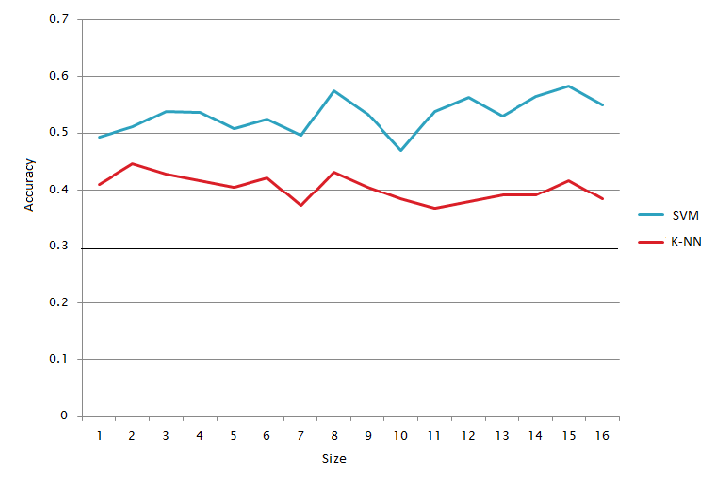
\includegraphics[scale = 0.4]{Scale_eff.png}
  \caption{Rescaling does not have much effect on classification }
\end{figure}


\subsection{Feature Extraction}
In this section, we describe some of the features that we used for the image classification task. All of these features were supposedly helpful in the classification task, as reflected in the references and thus we chose to use the following features as input to the classifiers. Note that we have used varied combinations of features and present results in the results sections with multiple combination of features fed into multiple classifiers. The features we considered include \\
\subsubsection{Haralick Features}
This is a set of 14 statistics that describe the texture of an image. These are calculated from co-occurrence matrix of the image. The co-occurrence matrix is $N_g${\bf X}$N_g$ matrix, where $N_g$ is the  number of distinct pixel values observed in the image. The (i,j) element in the matrix gives the probability of j$^{th}$ pixel value being adjacent to a pixel with i$^{th}$value. 

\subsubsection{Zoning Features}
Zoning is a method in which the image is split into multiple zones and features are then calculated for each of the zones. The features could be number of strokes, pixel count, histogram or any other feature. We calculate the number of dark pixels in a zone as a zonal feature. The effect of zoning is displayed in the plot below. The minimum error is obtained for 8 {\bf X} 8 zones in case of SVMs, and thus we continued to use this in further set of experiments. 
\begin{figure}[h]
  \centering
    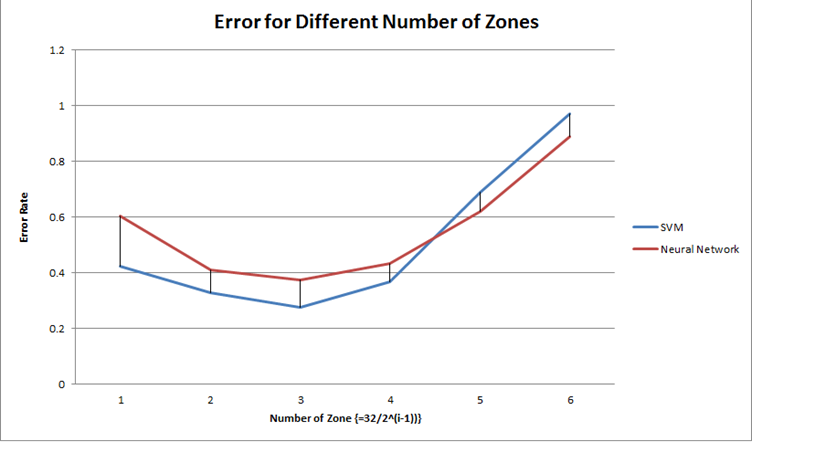
\includegraphics[scale = 0.4]{Zones_eff.png}
  \caption{Accuracy against combination of features }
\end{figure}

\subsubsection{Eccentricity}
Eccentricity of the image is a scalar quantity that specifies the eccentricity of the ellipse that has the same second-moments as the image.

\subsubsection{Raw Moment}
Harshit, i could not understand what to write from wiki page. Please you fill this section

\subsubsection{Covariance}
This corresponds to covariance of the matrix of the pixel values of the image.

\subsubsection{Contour}
This is a feature is constructed by calculating the distance of first dark pixel from each pixel on the image boundary in a direction perpendicular to the edge. This gives a vector of size 4$N$ for $N{\bf X}N$ image. This essentially captures the shape of the boundary that bounds the digits in images.
  
\subsubsection{Histogram}
This is a vector of size 2$N$ for $N{\bf X}N$ image. Each value represents the number of dark pixels set in row or column corresponding to that component in the vector.

\subsubsection{Thirteen Point Features}
Sayantan please reply back with what to write here. I forgot the 13 ways to dividing the image.

\subsubsection{Holes}
This represents the number of closed loops formed in the image. For example, a `1' has no loops, a `0' has one closed loop, `8' has two closed loops.

\section{Experimental Results}
As mentioned earlier, we carried out a set of experiments by using multiple combinations of above mentioned features against the following classification techniques. SVMs give the best accuracy amongst all the classifiers we have tried. The results over various feature combinations are given in the following graphs\\
\subsection{Support Vector Machines}
We used the SMO algorithm for multiclass classification which does one versus one SVM based binary classification. SVMs give the best result among all the classification techniques that we have tried. The accuracy obtained for various combination is plotted in the figures below. 
\begin{figure}[h]
  \centering
    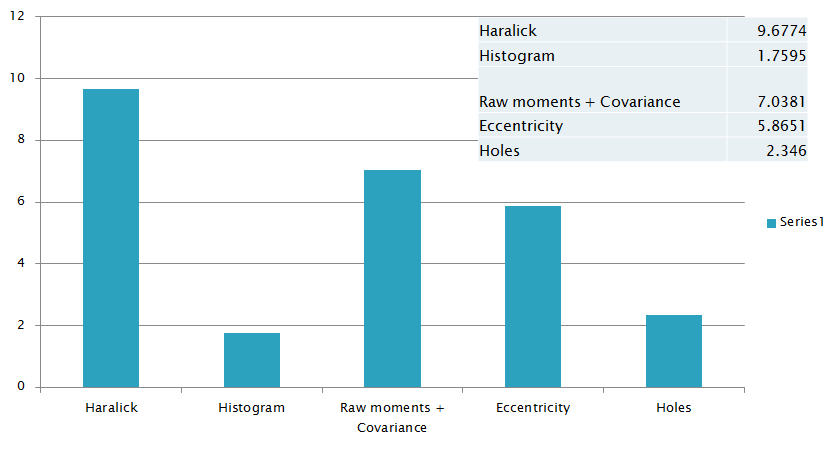
\includegraphics[scale = 0.4]{SVM_ind.png}
  \caption{Accuracy against individual features }
\end{figure}

\begin{figure}[h]
  \centering
    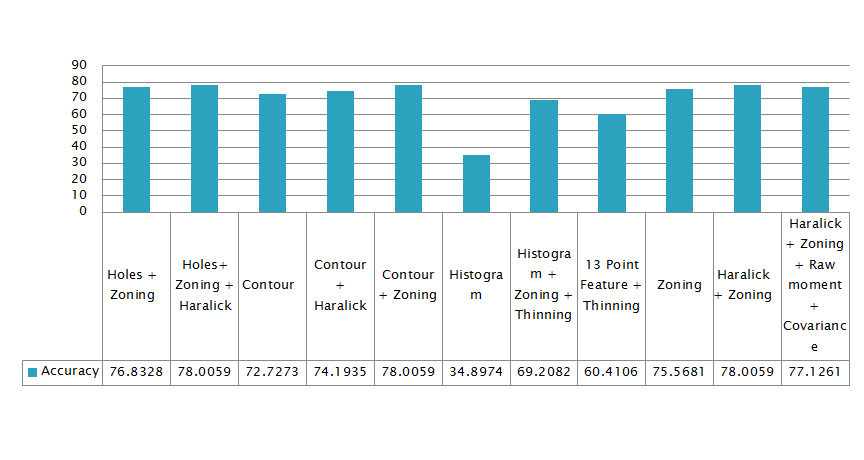
\includegraphics[scale = 0.4]{SVM_diff.png}
  \caption{Accuracy against combination of features }
\end{figure}

\begin{figure}[h]
  \centering
    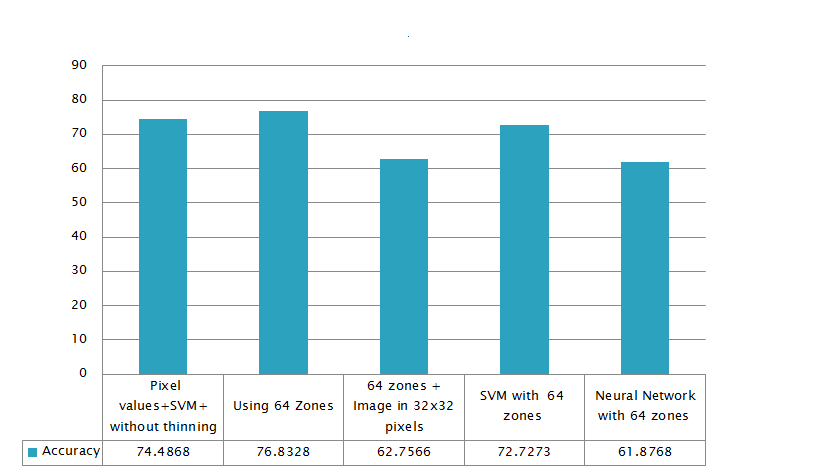
\includegraphics[scale = 0.4]{SVM_diff_2.png}
  \caption{Accuracy against combination of features }
\end{figure}

We used the polynomial kernel of degree one in the SVMs. We also varied the complexity parameter of the SVM to observe the effect on classification. The features used include zoning, haralick features and eccentricity on non thinned images. The effect of the parameter is shown in the following plot. 

\begin{figure}[h]
  \centering
    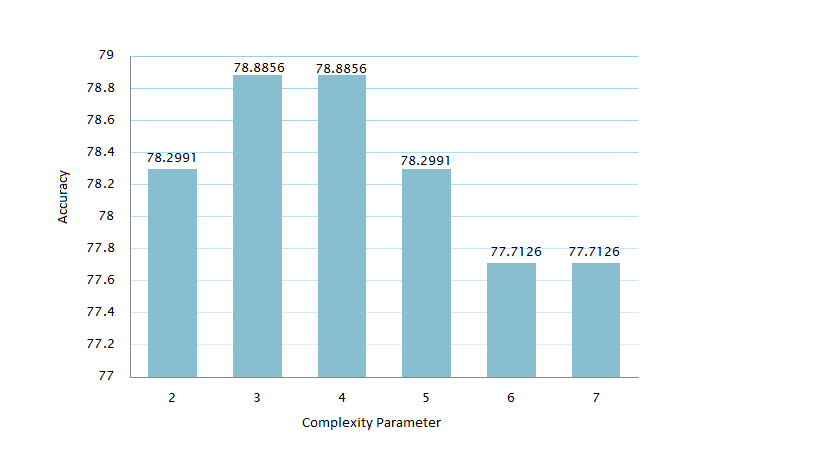
\includegraphics[scale = 0.4]{SVM_C_eff.png}
  \caption{Effect of complexity parameter }
\end{figure}

\subsection{K Nearest Neighbors}
The feature vector used for the classification using this model comprised of harlick features, eccentricity and zoning features. We varied the $K$ to observe the effect on classification. The variation is depicted in the figure below.

\begin{figure}[h]
  \centering
    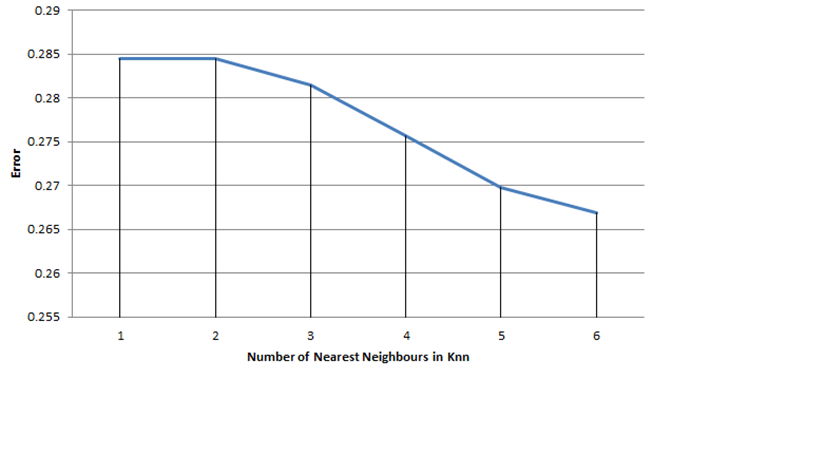
\includegraphics[scale = 0.5]{knn_n_eff.png}
  \caption{Variation of  error with K}
\end{figure}

\subsection{Neural Nets}
We made an attempt at the classification task using the Neural Nets. We tried single and two hidden layers in the network using the zoning, haralick, raw moments and eccentricity features. The accuracy obtained is plotted as below
\begin{figure}[h]
  \centering
    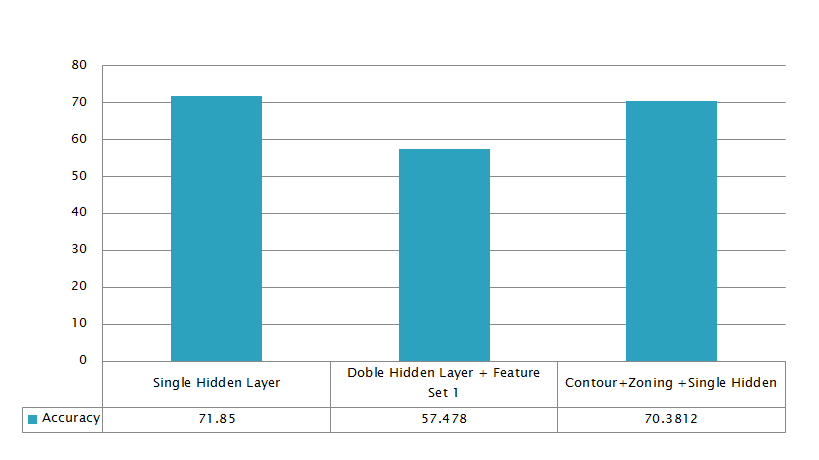
\includegraphics[scale = 0.5]{Neural_diff.png}
  \caption{Neural Nets with different layer and feature combination}
\end{figure}

\subsection{Random Forests}
We achieved an accuracy of 68.03\% using zoning features with random forests. An accuracy of 77.71\% was achieved using contour features and zoning features with random classifiers.

\section{Conclusion}
The highest accuracy achieved was 78.8\% using zoning ,eccentricity and haralick features with SVMs. Also based upon the above described set of experiments, we conclude that Zoning and Haralick Features have been influential in the classification task.


\begin{thebibliography}{0}
\bibitem{1} MNIST Database of handwritten digits. 
\emph{http://yann.lecun.com/exdb/mnist}
\bibitem{2} Connected Components. 
\emph{https://courses.cs.washington.edu/courses/cse576/ \\ 02au/homework/hw3/ConnectComponent.java}
\bibitem{3}Haralick Features. 
\emph{http://murphylab.web.cmu.edu/publications/boland/bo \\ land\_node26.html}
\bibitem{4}Zhabg Suen Thinning Algorithm. 
\emph{http://nayefreza.wordpress.com/2013/05 \\ /11/zhang-suen-thinning-algorithm-java-implementation/}
\bibitem{5}JFeatureLib. 
\emph{https://code.google.com/p/jfeaturelib/}
\end{thebibliography}
\end{document}